%!TEX root = ../thesis.tex
\newchap{Theoretical framework}\label{sec:TH}
\minitoc
\section{The Standard Model of particle physics}

The Standard Model of particle physics (SM) is a quantum field theory (QFT) that describes all the fundamental forces known beside gravity: the electromagnetic, the strong and the weak force. \\
The QFT is a framework that combines quantum mechanics, classical field theory and special relativity, allowing us to describe a particle as the excitation of a quantum field or, more formally, with an irreducible representation of the Poisson group that is characterized by the mass, spin, and additional quantum numbers of the particle.
Such theories are characterized by a Lagrangian density $\Lg{}$ that must be Lorentz invariant, must respect locality and must be renormalizable, \ie the perturbative expansions of the amplitudes must converge. \\
In the SM, additional local symmetries (Gauge symmetries) are imposed to describe the interactions between particles and, according to the Noether theorem \cite{NoetherInvarianteVariationsprobleme}, for each global symmetry a conserved charge arises.

\subsubsection*{Particles of the Standard Model}
Particles are divided into two main categories: fermions and bosons. 
Fermions are particles with half integer spin that obey to the Fermi-Dirac statistics and to the Pauli principle. 
Furthermore, each fermion has an antiparticle with the same mass but opposite quantum numbers.\\
Bosons are particles with integer spin that obey the Bose-Einstein statistics. In the SM there are the vector bosons (spin 1), the mediators of the forces, and the Higgs boson, the only scalar boson of the SM (spin 0). All the particles of the SM and their properties are summarized in \Fig{fig:SMpart}.



\begin{figure}[h!]
    \centering
    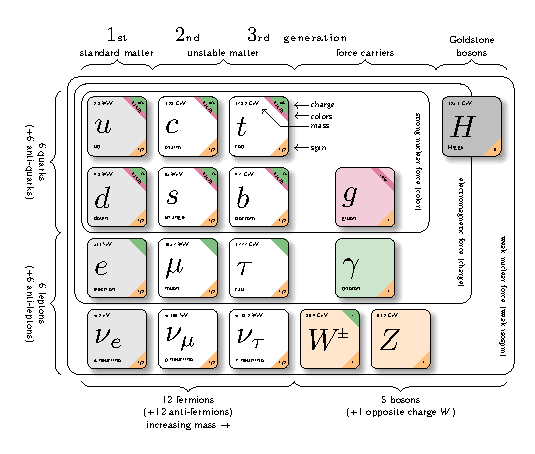
\includegraphics[width=1\linewidth]{fig/chap02-theory/SMpart.pdf}
    \caption{Fundamental particles of the Standard Model \cite{BurgardCarstenStandardExample}}
    \label{fig:SMpart}
\end{figure}

%commented
\iffalse
\paragraph*{Interactions}
The three fundamental interactions described by the SM are the electromagnetic, the strong and the weak force.\\
Each interaction has a Gauge boson that arises from a symmetry group.\\
The \emph{electromagnetic interaction} is described by the quantum electrodynamics (QED) \cite{FeynmanQED:Matter}, a \U{1} Gauge theory, and is mediated by the photon.\\
The \emph{strong interaction} is described by the quantum chromodynamics (QCD) \cite{Chromodynamics1995QUANTUMCHROMODYNAMICS} through the \SU{3} group.\\

\fi

\paragraph*{Fermions}
Fermions are divided into leptons and quarks, both divided in 3 generations, for a total of 12 fermions.\\
\emph{Quarks} are the constituents of the hadrons. They have a fractional electric charge and a color charge (and an anticolor charge for the antiquarks).\\
Quarks are divided into up-type quarks (up, charm, and top) with an electric charge of $Q=2/3$ and into down-type quarks (down, strange and bottom) with an electric charge of $Q=-1/3$.
One of the main properties of the QCD is the color confinement: isolated particles must be color singlets, so free quarks can't be observed because they hadronize (see sec. \ref{sub:QCD}).
The only exception is the top quark that decays before the hadronization due to its short lifetime.\\
Furthermore, weak interactions don't couple identically with all the flavours, but down-type quarks flavour are mixed according to the unitary CKM matrix.\\
\emph{Leptons} are the electron (\Pe), the muon (\PGm), the tau (\PGt) and their respective neutrinos (\PGne, \PGnGm, \PGnGt).
A charged lepton and its respective neutrino represent a generation of leptons with a corresponding family lepton flavor number $L_{\ell_i}=n_{\ell_i}-n_{\PAl_i}$ that, in SM, is conserved together with the total lepton number $L=n_\ell-n_\PAl$.
The leptons participate in all the interactions except the strong force.\\


\subsection{Gauge theories and the QED}\label{sub:gauge_qed}
\paragraph*{Fermion free fields}
The Lagrangian (density) for a free fermion field is the Dirac Lagrangian
\begin{equation}\label{eq:Dirac}
\mathcal{L}_{\text{Dirac}}=i\bar{\psi}\gamma^{\mu}\partial_{\mu}\psi-m\bar{\psi}\psi
\end{equation}
where $\aff{\psi}{}=\ff{\psi}{}^\dagger\gamma^0$ is the adjoint Dirac spinor, and $\gamma^\mu$ are the 4 Dirac matrices that obey the Clifford algebra $\{\gamma^\mu,\gamma^\nu\}=2\eta^{\mu\nu}$\\
The corresponding equation of motion has two solutions: the one with the positive energy represents the fermion field, the one with the negative energy represents the anti-fermion field.\\
Dirac spinors are $\left( \frac{1}{2} \right)$ representations of the Lorentz group $SO^+(1,3)$ that can be decomposed into the $\SU[L]{2} \oplus \SU[R]{2}$ group.\\
Using this different representation, Dirac spinors can be described in the so-called chiral basis $\psi=\left(\psi_L,\psi_R \right)$ where $\psi_{L/R}$ are called left/right Weyl spinors and are respectively the $\left(\frac{1}{2},0\right)$ and the $\left(0,\frac{1}{2}\right)$ representations of the $\SU{2} \oplus \SU{2}$ group.\\
The chirality operator $\gamma^5=i\gamma^0\gamma^1\gamma^2\gamma^3$ anti-commutes with all the gamma matrices and commute with the Dirac Hamiltonian only if the mass is zero, so it is a good quantum number only for massless particles.\\
The chirality plays an important role in the weak interaction, as described in sec. \ref{sub:weak}
\paragraph*{Gauge theories}
The standard procedure to introduce a global symmetry in the Lagrangian and a Gauge boson field is the following:
\begin{enumerate}
    \item Introduce a local symmetry based on a Lie group:
    \begin{equation}\label{eq:spinor_gauge}
        \psi(x) \to \psi^\prime (x)=g(x) \psi(x) = e^{i \alpha_a(x) t^a}\psi(x)
    \end{equation}
    where $g(x)$ is a representation of the group and $t^a$ its generators
    \item Replace the partial derivatives $\partial_\mu$ with the covariant derivative $D_\mu$
    \begin{equation}\label{eq:covariant_derivative}
        D_{\mu}\psi(x)=\left(\partial_{\mu}-i g\,A_{\mu}^{a}(x)\,t^{a}\right)\psi(x)\;
    \end{equation}
    where $g$ is the coupling constant between the fermion field and the Gauge fields and $A^a_\mu$ the Gauge fields 
    \item The covariant derivative should transform according to the Gauge group $D_\mu \psi(x)\to g(x) D_\mu \psi(x)$ and, with some calculation, it is possible to find that the Gauge field transform as the following under the action of the Gauge group
    \begin{equation}\label{eq:gauge_field_transformation}
        A_{\mu}(a)\rightarrow g(x)A_{\mu}(x)g^{-1}(x)-\frac i g\,\bigg(\partial_{\mu} g(x)\bigg) g^{-1}(x)\,
    \end{equation}
    where $A_\mu=A_\mu^a(x)t^a$
    \item The final Lagrangian now has a global invariance for the Gauge group and, according to the Noether theorem, there is a conserved charge. Furthermore, in this procedure, another vector massless field arises.
\end{enumerate}
\paragraph*{Quantum electrodynamics}
The simplest case of a Gauge theory is the quantum electrodynamics (QED) \cite{FeynmanQED:Matter} in which the Gauge group is \U{1}, a commutative group for which holds $g(x)g(y)=g(y)g(x)$\\
The fundamental representation of the \U{1} group is $g(x)=e^{i \alpha(x)}$, \ie a local phase.\\
Imposing the \U{1} invariance on the Dirac Lagrangian, we obtain the QED Lagrangian.
\begin{equation}\label{eq:QED}
    \Lg{QED}=i\bar{\psi}\gamma^{\mu}(\partial_{\mu}+i q A_{\mu})\psi-m\bar{\psi}\psi-\frac{1}{4}F^{\mu\nu}F_{\mu\nu}
\end{equation}
where $A_\mu$ is the photon field, $q$ the elementary electron charge and $F_{\mu\nu}=\partial_\mu A_\nu-\partial_\nu A_\mu$ the electromagnetic tensor\\
In the SM, all the fermions, except the neutrinos, have an electric charge and are involved in the electromagnetic interactions.\\


\subsection{Quantum chromodynamics}\label{sub:QCD}
The quantum chromodynamics (QCD) is the \SU{3} Gauge theory that describes the strong interaction and involves gluons and quarks, bonding together into hadronic states.
The quantum number related to strong interaction is the color charge.
Applying the gauging technique described in the section \ref{sub:gauge_qed} is possible to obtain the QCD Lagrangian.
\begin{equation}\label{eq:QCD}
    \Lg{QCD}=-i g_{s}\bar{\psi}\gamma^{\mu}\lambda_{a}\psi G_{\mu}^a-\frac{1}{4}G_{a}^{\mu\nu}G_{\mu\nu}^a
\end{equation}
where \(G_{\mu\nu}^{a}=\partial_{\mu}G_{\nu}^{a}-\partial_{\nu}G_{\mu}^{a}-g_{s}f^{a b c}G_{\mu}^{b}G_{\nu}^{c}\) is the corresponding of the electromagnetic tensor for the strong force, $\lambda_a$ are the \SU{3} generators, and $f^{abc}$ the \SU{3} structure constants.\\
Each quark carries a color charge and each anti-quark an anticolor charge and, since \SU{3} has 8 generators, 8 gluons exist (or just one gluon that can carry one of 8 possible couples of color-anticolor).\\
There are significant differences with the QED to the non-abelianity of \SU{3}:
\begin{itemize}
    \item \textbf{Gluon self-coupling}: gluons can interact with each other.
    \item \textbf{Asymptotic freedom}: the coupling strength decreases with the energy, \ie at large energy scales the quarks become quasi-free.\\
    The coupling constant of the strong interaction depends on the energy scale \cite{Deur2016TheCoupling}
    \begin{equation}\label{eq:alphas_run}
        \alpha_S(\mu^2)\propto \frac{1}{\ln \left( \frac{\mu^2}{\Lambda_{\text{QCD}}^2}\right)}        
    \end{equation}
    Where $\Lambda_{QCD}\approx 200 \MeV$ and $\mu$ is the energy scale.\\
    When $\mu \gg \Lambda_{QCD}$, strong interactions can be described using perturbative techniques (pQCD) but, at low-energy scales, the QCD is non perturbative and that leads to the third property of the QCD
    \item \textbf{Color confinement}: At low-energy scales, the strong coupling is so large that quarks are always bounded in color singlets and isolated quarks can't be observed.\\
    This is also why the strong force has a limited range, while the electromagnetic force has an infinite range.
\end{itemize}

\subsection{Electroweak unification}\label{sub:weak}
\paragraph*{Weak interactions}
The weak interaction was first introduced by Enrico Fermi to explain the $\beta$ decay through the 4 point Fermi interaction \cite{Fermi1934Tentativo} and is the only force that involves all the fermions and that violates the parity and the charge parity conservation. \\
The quantum number related to the weak interaction is the weak isospin, generated by the \SU{2} gauge group that creates 3 gauge bosons: the $W^\pm$ and the $Z$ bosons.\\
Trying to build the weak Lagrangian only using the gauging technique described in the section \ref{sub:gauge_qed} doesn't work in this case for different reasons:
\begin{itemize}
    \item The W boson and the Z boson would have the same coupling to the fermions, while experimentally this was disproven. To address this problem, the weak interaction was unified to the electromagnetic interaction.
    \item The W/Z bosons are proven to be massive bosons, while gauge bosons are always massless. The massive term can't be added arbitrary to the Lagrangian because such a theory would be non renormalizable, so they have to be added through the Higgs mechanism as described in the section \ref{sub:SM}.\\
    The non-zero W/Z mass  is also the cause why the weak interactions have a finite range, given that the weak interactions are suppressed by the weak propagator $1/(q^2-M_{W/Z}^2)$.
    \item The weak interaction doesn't couple identically with all the quarks, but the down-type flavours are mixed by the Cabibbo-Kobayashi-Maskawa (CKM) matrix \cite{Kobayashi1973CP-ViolationInteraction}, as described in section \ref{sec:CKM}. The elements of the CKM matrix are complex, and this leads to the CP violation.
    \item To introduce the parity violation in the Lagrangian, the $\gamma^\mu$ in the interaction term of the Lagrangian has to be replaced with $\gamma^\mu \left(1-\gamma^5 \right)/2 $.\\
    The term $(1-\gamma^5)/2$ is the left chirality projector, and this implies that weak interaction couples only with the left part of the spinor. This will turn to be true only for charged weak interactions, while for neutral weak interactions, the mixing between the photon and the Z boson in the electroweak (EW) unification process will reintroduce the coupling with the right spinors.
\end{itemize}

\paragraph*{Electroweak unification}\label{sub:EW}
The electromagnetic and weak interactions were unified in the Glashow-Weinberg-Salam theory \cite{Weinberg1967ALeptons,Salam1964ElectromagneticInteractions,Glashow1961PartialInteractions} based on the $\SU{2} \otimes \U(1)$ symmetry group.\\
We start defining left-handed doublets and right-handed singlets
\begin{align}
    Q_{L,i}=\left({u_{L,i}}\atop{d_{L,i}}\right), \quad u_{R,i},\quad d_{R,i} \\
    \mathcal{L}_{L,i}=\left(\begin{array}{l}{{\nu_{L,i}}}\\ {{\ell_{L,i}}}\end{array}\right),\quad\ell_{R,i}
\end{align}
so left-handed particles organize in $\SU{2}$ doubles while right-handed particles in $\SU{2}$ singlets.
The gauge invariant Lagrangian for the group $\SU{2}\otimes\U{1}$ is:
\begin{equation}\label{eq:EWK_preunification}
{\mathcal{L}}=i\overline{{{L}}}\gamma^{\mu}D_{\mu}L+\overline{{{R}}}i\gamma^{\mu}D_{\mu}R-\frac{1}{4}B^{\mu\nu}B_{\mu\nu}-\frac{1}{4}W_{a}^{\mu\nu}W_{\mu\nu}^{a}
\end{equation}
where
\begin{itemize}
    \item L and R are the left doublets and the right singlets
    \item $D_{\mu}=\partial_{\mu}-i{\frac{g^{\prime}}{2}}\hat{Y}B_{\mu}-i g\hat{T}_{i}W_{\mu}^{i}$ is the covariant derivative
    \item $\hat{Y}$ is the \U{1} generator (the hypercharge operator)
    \item $\hat{T}_i$ are the three \SU{2} generators (weak isospin operators)
    \item $B^{\mu\nu}=\partial_{\mu}B_{\nu}-\partial_{\nu}B_{\mu}$, where $B_\mu$ is the \U{1} gauge field
    \item $W_{\mu\nu}^{i}=\partial_{\mu}W_{\nu}^{i}-\partial_{\nu}W_{\mu}^{i}-g\epsilon^{i j k}W_{\mu}^{j}W_{\nu}^{k}$ where $W^i_\mu$ are the 3 \SU{2} gauge fields and $\epsilon^{ijk}$ the \SU{2} structure constants. 
\end{itemize}
The experimental observed W, Z and $\gamma$ bosons can be expressed as a linear combination of the defined gauge fields.
\begin{gather}
    W_\mu^{\pm}=(W^1_\mu\pm i W^2_\mu)/\sqrt{2}\\
    \db{A_\mu}{Z_\mu}=\left(\begin{array}{l l}{{\cos\theta_{W}}}&{{\sin\theta_{W}}}\\ {{-\sin\theta_{W}}}&{{\cos\theta_{W}}}\end{array}\right)\db{B_\mu}{W^3_\mu}
\end{gather}
where the mixing angle $\theta_W$ is the Weinberg angle, and it can be proven that $\cos(\theta_W)=m_W/m_Z$.\\
After the mixing, we can break the electroweak Lagrangian into different pieces:
\begin{equation}\label{eq:EWK}
    \Lg{EWK}=\Lg{kin}+\Lg{QED}+\Lg{wcc}+\Lg{wnc}+\Lg{gauge}
\end{equation}

\begin{itemize}
    \item  $\Lg{kin}$ is the fermions kinetic term
    \item $\Lg{QED}$ is the interaction term of the QED Lagrangian described in section \ref{sub:gauge_qed}
    \item $\Lg{wcc}$ is the interaction term of the weak charged currents
    \begin{equation}
        {\mathcal{L}}_{wcc}\,=\,\frac{g}{2{\sqrt{2}}}\,\left\{W_{\mu}^{\dagger}\,\bar{L}\gamma^{\mu}(1-\gamma_{5})L+\,\dots \right\}
    \end{equation}
    the charged weak interactions preserve the vector-axial (V-A) structure, and this implies that the $W^\pm$ bosons interact only with the left doublets.\\
    Furthermore, the weak interactions mix the down-type quark flavours so the terms that involve quarks have to include a unitary matrix, the CKM matrix. (see sec.\ref{sec:CKM})
    \begin{equation}
        \Lg{wcc}^q=-\frac{g}{\sqrt{2}}(\overline{{{u}}}_{L},\overline{{{c}}}_{L},\overline{{{t}}}_{L})\gamma^{\mu}W_{\mu}^{+}V_{\mathrm{CKM}}\tb{d_{L}}{s_{L}}{b_L}+\dots
    \end{equation}
    This also does not allow the presence of flavour changing neutral currents (FCNC).
    \item $\Lg{wnc}$ is the interaction term of the weak neutral currents,
    \begin{equation}
        \Lg{wnc}=\frac{e}{2\sin\theta_{W}\cos\theta_{W}}\,Z_{\mu}\sum_{f}\,\bar{f}\gamma^{\mu}(v_{f}-I^3_{f}\gamma_{5})\,f\;
    \end{equation}
    where $I^3_f$ is the weak isospin of the fermion and $v_f=I^{3}_{f}\left(1-4|Q_{f}|\sin^{2}\theta_{W}\right)$.
    Unlike the W boson, the Z boson interacts both with the left and the right part of the spinor with different couplings depending on the isospin and the charge of the fermion 
    \item $\Lg{gauge}$ is the kinematic part of the Lagrangian related to the Gauge bosons
\end{itemize}


\subsection{The spontaneous symmetry breaking}\label{sub:SM}
The EW Lagrangian in \Eq{eq:EWK} does not include both the fermions and the boson masses.
In the SM, the W/Z masses are generated by the Higgs-Brout-Englert mechanism \cite{Higgs1964BrokenBosons,Englert1964BrokenMesons}.
Starting from the  $\SU[C]{3} \otimes \SU[L]{2} \otimes \U[Y]{1}$ Lagrangian,
\begin{equation}
    \Lg{}=\Lg{kin}+\Lg{QCD}+\Lg{EWK}
\end{equation}
we add another term introducing a scalar complex doublet field
\begin{equation}\label{eq:Higgs_preSSB}
    \Lg{H}=(D^{\mu}\phi)^{\dagger}(D_{\mu}\phi)-\frac{1}{2}\mu^{2}(\phi^{\dagger}\phi)-\frac{1}{4}\lambda(\phi^{\dagger}\phi)^{2}
\end{equation}
where $D_\mu$ is the electroweak covariant derivative defined in \Eq{eq:EWK_preunification} and $\mu^2<0$.
The last 2 terms form the Higgs potential $V(\phi)$, represented in \Fig{fig:HiggsPotential}.

The minimum of $V(\phi)$ is not unique, and the choice of a specific minimum for $\phi$ leads to the spontaneous symmetry breaking (SSB) of the $\SU{3} \otimes \SU{2} \otimes \U{1}$ group into the $\SU{3} \otimes \U{1}$ group.\\
A convenient choice is to pick the ground state of $\phi$ as
\begin{equation}
    \langle\phi\rangle=\frac{1}{\sqrt{2}}\db{0}{v}=\frac{1}{\sqrt{2}}\db{0}{\sqrt{\frac{-\mu^2}{\lambda}}}
\end{equation}
Developing the Lagrangian in \Eq{eq:Higgs_preSSB} around this minimum, we can redefine the scalar doublet as
\begin{equation}\label{eq:higgs_intro}
    \phi=\db{0}{v+H(x)}
\end{equation}
where $H(x)$ is the scalar field corresponding to the Higgs boson. \\
Replacing \Eq{eq:higgs_intro} into the \Eq{eq:Higgs_preSSB} the W/Z bosons acquire a mass term with
\begin{gather}
    M_{W^\pm}=\frac{1}{2}gv\\
    M_Z=\frac{M_{W^\pm}}{\cos (\theta_W)}
\end{gather}
This also generates the Higgs boson mass $m_H=\sqrt{2\lambda}\mu$, the interactions between the Higgs boson and the vector bosons and the Higgs self-interactions.
\begin{figure}[h!]
    \centering
    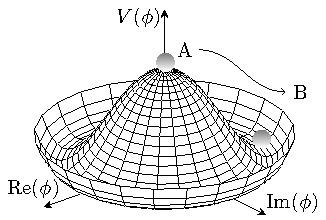
\includegraphics[width=0.95\linewidth]{fig/chap02-theory/higgs.pdf}
    \caption{Higgs potential \cite{HiggsTikZ.net}}
    \label{fig:HiggsPotential}
\end{figure}\\
\paragraph*{Fermion masses}
The Lagrangian $\Lg{}=\Lg{kin}+\Lg{QCD}+\Lg{EWK}+\Lg{H}$ does not contain the fermion masses yet.\\
The mass terms of the Dirac Lagrangian (\Eq{eq:Dirac}) can't be added directly because the term \(-m \bar{\psi} \psi\) is not invariant under $\SU{2}\otimes \U{1}$.
This problem can be addressed by introducing the Yukawa interaction between fermions and the Higgs field
\begin{equation}
    \Lg{Yukawa}=-\left(g_{i j}^{d}\bar{Q}_{L,i}\phi d_{R,j}+g_{i j}^{u}\bar{Q}_{L,i}(i\sigma^{2}\phi^{\dagger})u_{R,j}+g_{i j}^{\ell}\bar{\mathcal{L}}_{L,i}\phi\ell_{R,j}\right)+h.c.
\end{equation}
After the SSB, the fermions masses arise from the Yukawa interaction.
\begin{gather}
    \Lg{masses}=-M_{i j}^{\ell}\bar{\ell}_{L,i}\ell_{R,j}-M_{i j}^{d}\bar{d}_{L,i}d_{R,j}-M_{i j}^{u}\bar{u}_{L,i}u_{R,j}\\
    M^{\ell,d,u}=\frac{v}{\sqrt{2}}g^{\ell,d,u}
\end{gather}
At this point, the SM is complete.\\ 
A summary of all the particles of the SM and their quantum numbers is in Tab. \ref{tab:SM}

%!TEX root = ../thesis.tex

% TABLE: SM Summary
%   https://en.wikipedia.org/wiki/File:Electroweak.svg
%   https://commons.wikimedia.org/wiki/File:Standard_Model.svg
%   https://en.wikipedia.org/wiki/Mathematical_formulation_of_the_Standard_Model#Field_content_in_detail
\begin{table}[h!]
\vspace*{-6mm}
\centering
\caption{
Summary of the representation and quantum numbers SM fields.
Bold numbers indicate the dimension of the representation under the respective gauge group.
}\label{tab:SM_symmetries}
\def\arraystretch{1.3}
\def\vsdb{\rule[-15pt]{0pt}{36pt}} % vertical space for doublet
\begin{tabular}{llc@{\extracolsep{\tabcolsep}}c@{\extracolsep{4pt}}c@{\extracolsep{\tabcolsep}}c@{\extracolsep{1.5\tabcolsep}}c}
  \hline
  %Field name  & Symbol      & $\SU[C]{3}$ & $\SU[L]{2}$ & $T_3$ & $\YW/2$ & $Q = T_3 + \YW/2$ \\
  \multirow{2}{*}{Field name}
        & \multirow{2}{*}{Symbol}
               & \multicolumn{2}{c}{Representations} & \multicolumn{3}{c}{Quantum numbers} \\
                 \cline{3-4}                           \cline{5-7}
        &      & $\SU[C]{3}$ & $\SU[L]{2}$ & $T_3$ & $\YW/2$ & $Q = T_3 + \YW/2$ \\
  \hline
  \vsdb % add vertical space above & below
  Quark doublet
        & $\ff{Q}{L} = \db{\ff{u}{L}}{[1pt]\ff{d}{L}}$
               & \textbf{3}  & \textbf{2} & $\db{+\frac{1}{2}}{[2pt]-\frac{1}{2}}$
                                                   & $+\frac{1}{6}$
                                                             & $\db{+\frac{2}{3}}{[2pt]-\frac{1}{3}}$ \\[2mm]
  Up-quark singlet
        & $\ff{u}{R}$  & \textbf{3}  & \textbf{1} & $+\frac{2}{3}$
                                                   & $+\frac{2}{3}$
                                                             & $+\frac{2}{3}$ \\
  Down-quark singlet
        & $\ff{d}{R}$  & \textbf{3}  & \textbf{1} & $-\frac{1}{3}$
                                                   & $-\frac{1}{3}$
                                                             & $-\frac{2}{3}$ \\
  \vsdb % add vertical space above & below
  Lepton doublet
        & $\ff{L}{L} = \db{\ff{\nu}{L}}{[1pt]\ff{e}{L}}$ 
                       & \textbf{1}  & \textbf{2} & $\db{+\frac{1}{2}}{[2pt]-\frac{1}{2}}$
                                                   & $-\frac{1}{2}$
                                                             & $\db{\phmin0}{-1}$ \\[2mm]
  Lepton singlet
        & $\ff{e}{R}$  & \textbf{1}  & \textbf{1} & $\phmin0$
                                                   & $-1$    & $-1$ \\
  \hline
  Gluon field
        & $G^a_\mu$    & \textbf{8}  & \textbf{1} & $\phmin0$
                                                   & $\phmin0$ & $\phmin0$ \\
  \rule[-19pt]{0pt}{42pt}% % add vertical space above & below
  Weak gauge field
        & $W^i_\mu = \db{W^+_\mu}{W^-_\mu\\W^3_\mu}$
                       & \textbf{1}  & \textbf{3} & $\db{+1}{-1\\\phmin0}$
                                                   & $\phmin0$ & $\db{+1}{-1\\\phmin0}$\\
  Hypercharge field
        & $B_\mu$
                       & \textbf{1}  & \textbf{1} & $\phmin0$
                                                   & $\phmin0$ & $\phmin0$ \\
%  Weak gauge bosons
%        & $\db{W^+_\mu}{W^-_\mu\\Z^0_\mu}$
%               & \textbf{1}  & \textbf{3} & $\db{+1}{-1\\0}$
%                                                   & \phmin0 & $\db{+1}{-1\\\phmin0}$\\
%  Photon
%        & $A^a_\mu$    & \textbf{1}  & \textbf{1} & $\phmin0$
%                                                   & $\phmin0$ & $\phmin0$ \\
  \hline
  \vsdb % add vertical space above & below
  Higgs doublet
        & $\Phi = \db{\phi^+}{[1pt]\phi^0}$
               & \textbf{1}  & \textbf{2} & $\db{+\frac{1}{2}}{[2pt]-\frac{1}{2}}$
                                                   & $+\frac{1}{2}$
                                                             & $\db{+1}{\phmin0}$ \\[2mm]
  \vsdb % add vertical space above & below
  Conjugate Higgs doublet
        & $\Phi^\mathrm{c} = \db{\phi^{0*}}{[1pt]\phi^-}$
               & \textbf{1}  & \textbf{2} & $\db{+\frac{1}{2}}{[2pt]-\frac{1}{2}}$
                                                   & $-\frac{1}{2}$
                                                             & $\db{\phmin0}{-1}$ \\[2mm]
  \hline
\end{tabular}
\label{tab:SM}
\end{table}


\section{The CKM matrix}\label{sec:CKM}
As already introduced, the weak interactions mix the down-type quarks with the Cabibbo-Kobayashi-Maskawa (CKM) matrix \cite{Cabibbo_angle,Kobayashi1973CP-ViolationInteraction}.
\begin{equation}
    \Lg{wcc}^q=-\frac{g}{\sqrt{2}}(\overline{{{u}}}_{L},\overline{{{c}}}_{L},\overline{{{t}}}_{L})\gamma^{\mu}W_{\mu}^{+}V_{\mathrm{CKM}}\tb{d_{L}}{s_{L}}{b_L}+\dots
\end{equation}
\begin{equation}
V_{C K M}=\left(\begin{array}{l l l}{{V_{u d}}}&{{V_{u s}}}&{{V_{u b}}}\\ {{V_{c d}}}&{{V_{c s}}}&{{V_{c b}}}\\ {{V_{t d}}}&{{V_{t s}}}&{{V_{t b}}}\end{array}\right)\,
\end{equation}
The CKM matrix is a $3 \times 3$ complex matrix, so it can be written in terms of 18 real parameters. The unitarity condition $V^\dagger V$ adds 8 constraints, and the 6 quark fields can absorb the phases defining a new common phase, so the number of parameters of the CKM is four.\\
These parameters can be  both determined through global fits that combine experimental data from different experiments, imposing the constraints of the standard model (\eg the unitarity), or can be measured independently \cite{PDG_2022}.\\
Measure all the parameters independently allows us to verify the unitarity of the CKM matrix that, if violated, can be a sign of new physics.\\
The $|V_{ud}|$ is the element measured with the highest precision through  the study of $\beta$ decays. The other $|V_{uq}|$ and $|V_{cq}|$ elements are measured through leptonic and semileptonic meson decays, but these kinds of measures are highly affected by theoretical uncertainties due to the non-perturbative nature of the strong interaction at low energy that bonds the quarks in the meson.
The $|V_{tq}|$ elements are not affected by theoretical uncertainties, but the QCD background of a hadron collider makes their measure really challenging and, at this time, an electron-positron collider with a sufficient energy in the center of mass to produce a top quark does not exist yet.
\\
\\
There are two common parametrizations of the CKM matrix: the standard parametrization and the Wolfenstein parametrization \cite{PDG_2022}.
The values of the parameters listed below are the ones obtained from the CKMfitter group through a global fit \cite{Charles2005CPFactories,Hocker2001AMatrix,PDG_2022}.
\paragraph*{Standard parametrization}
In the standard parametrization, the CKM matrix is expressed as the product of 3 rotation matrices with the addition of a phase.
\begin{equation}
    V_{C K M}=\left(\begin{array}{c c c c}{{1}}&{{0}}&{{0}}\\ {{0}}&{{c_{23}}}&{{s_{23}}}\\ {{0}}&{{-s_{23}}}&{{c_{23}}}\end{array}\right)\left(\begin{array}{c c c}{{c_{13}}}&{{0}}&{{s_{13}e^{-i\delta}}}\\ {{0}}&{{1}}&{{0}}\\ {{-s_{13}e^{i\delta}}}&{{0}}&{{c_{13}}}\end{array}\right)\left(\begin{array}{c c c}{{c_{12}}}&{{s_{12}}}&{{0}}\\ {{-s_{12}}}&{{c_{12}}}&{{0}}\\{{0}}&{0}&{1}\end{array}\right)
\end{equation}
where  $c_{ij}=\cos{\theta_{ij}}$, $s_{ij}=\sin(\theta_{ij})$ and $\delta$ is the phase responsible for the CP violation in weak interactions.\\
The values obtained by the CKMfitter group are the following
\begin{equation}
    \begin{array}{l l}{{\sin\theta_{12}=0.22500\pm0.00085\,,~~~~~}}&{{\sin\theta_{13}=0.00369\pm0.00011\,,}}\\ {{\sin\theta_{23}=0.04182_{-0.00074}^{+0.00067\,,}~~~~}}&{{\delta=1.144\pm0.027\,.}}\end{array}
\end{equation}


\paragraph*{Wolfenstein's parametrization}
Defining new four real parameters, 
\begin{gather}
    s_{12}=\lambda={\frac{|V_{u s}|}{\sqrt{|V_{u d}|^{2}+|V_{u s}|^{2}}}} ,\\
    s_{23}=A\lambda^{2}=\lambda|\frac{V_{c b}}{V_{u s}}|,\\
    s_{13}e^{i\delta}=A\lambda^{3}(\rho+i\eta)=\frac{A\lambda^{3}(\bar{\rho}+i\bar{\eta})\sqrt{1-A^{2}\lambda^{4}}}{\sqrt{1-\lambda^{2}}\left[1-A^{2}\lambda^{4}(\bar{\rho}+i\bar{\eta})\right]}\,
.
\end{gather}
the Wolfenstein parametrization shows clearly the order of magnitude of the different elements in powers of $\lambda$
\begin{equation}
    V_{C K M}\simeq\left(\begin{array}{c c c}{{1-\frac{\lambda^{2}}2\ \ \ }}&{{\lambda}}&{{\lambda^{3}(\rho-i\eta)}}\\ {{-\lambda}}&{{1-\frac{\lambda^{2}}2\ \ \ }}&{{A\lambda^{2}}}\\ {{A\lambda^{3}(1-\rho-i\eta)}}&{{-A\lambda^{2}}}&{{1}}\end{array}\right)+{\cal O}(\lambda^{4}).
\end{equation}
The CKMfitter group performed a global fit for this parametrization as well.
\begin{equation}
    \begin{array}{l l}{{\lambda=0.22500\pm0.00067\,,~~~~}}&{{A=0.826_{-0.015}^{+0.018}\,,}}\\ {{\bar{\rho}=0.159\pm0.010\,{,~~~}}}&{{\bar{\eta}=0.348\pm0.010\,.}}\end{array}
\end{equation}
\paragraph*{Unitarity triangle}
The six unitarity constraints of the CKM matrix are:
\begin{gather}
    \sum_i V_{ij}V_{ik}^*=\delta_{jk}\\
    \sum_j V_{ij}V_{kj}^*=\delta_{ik}
\end{gather}
These constraints can be represented in the complex $(\bar{\rho},\bar{\eta})$ plane in a triangle with vertexes $(0,0), (1,0), (\bar{\rho},\bar{\eta})$ \Fig{fig:triangle}.\\
The area of the unitarity triangle is also a measure of the CP violation of the weak interactions.
\begin{figure}[h]
    \centering
    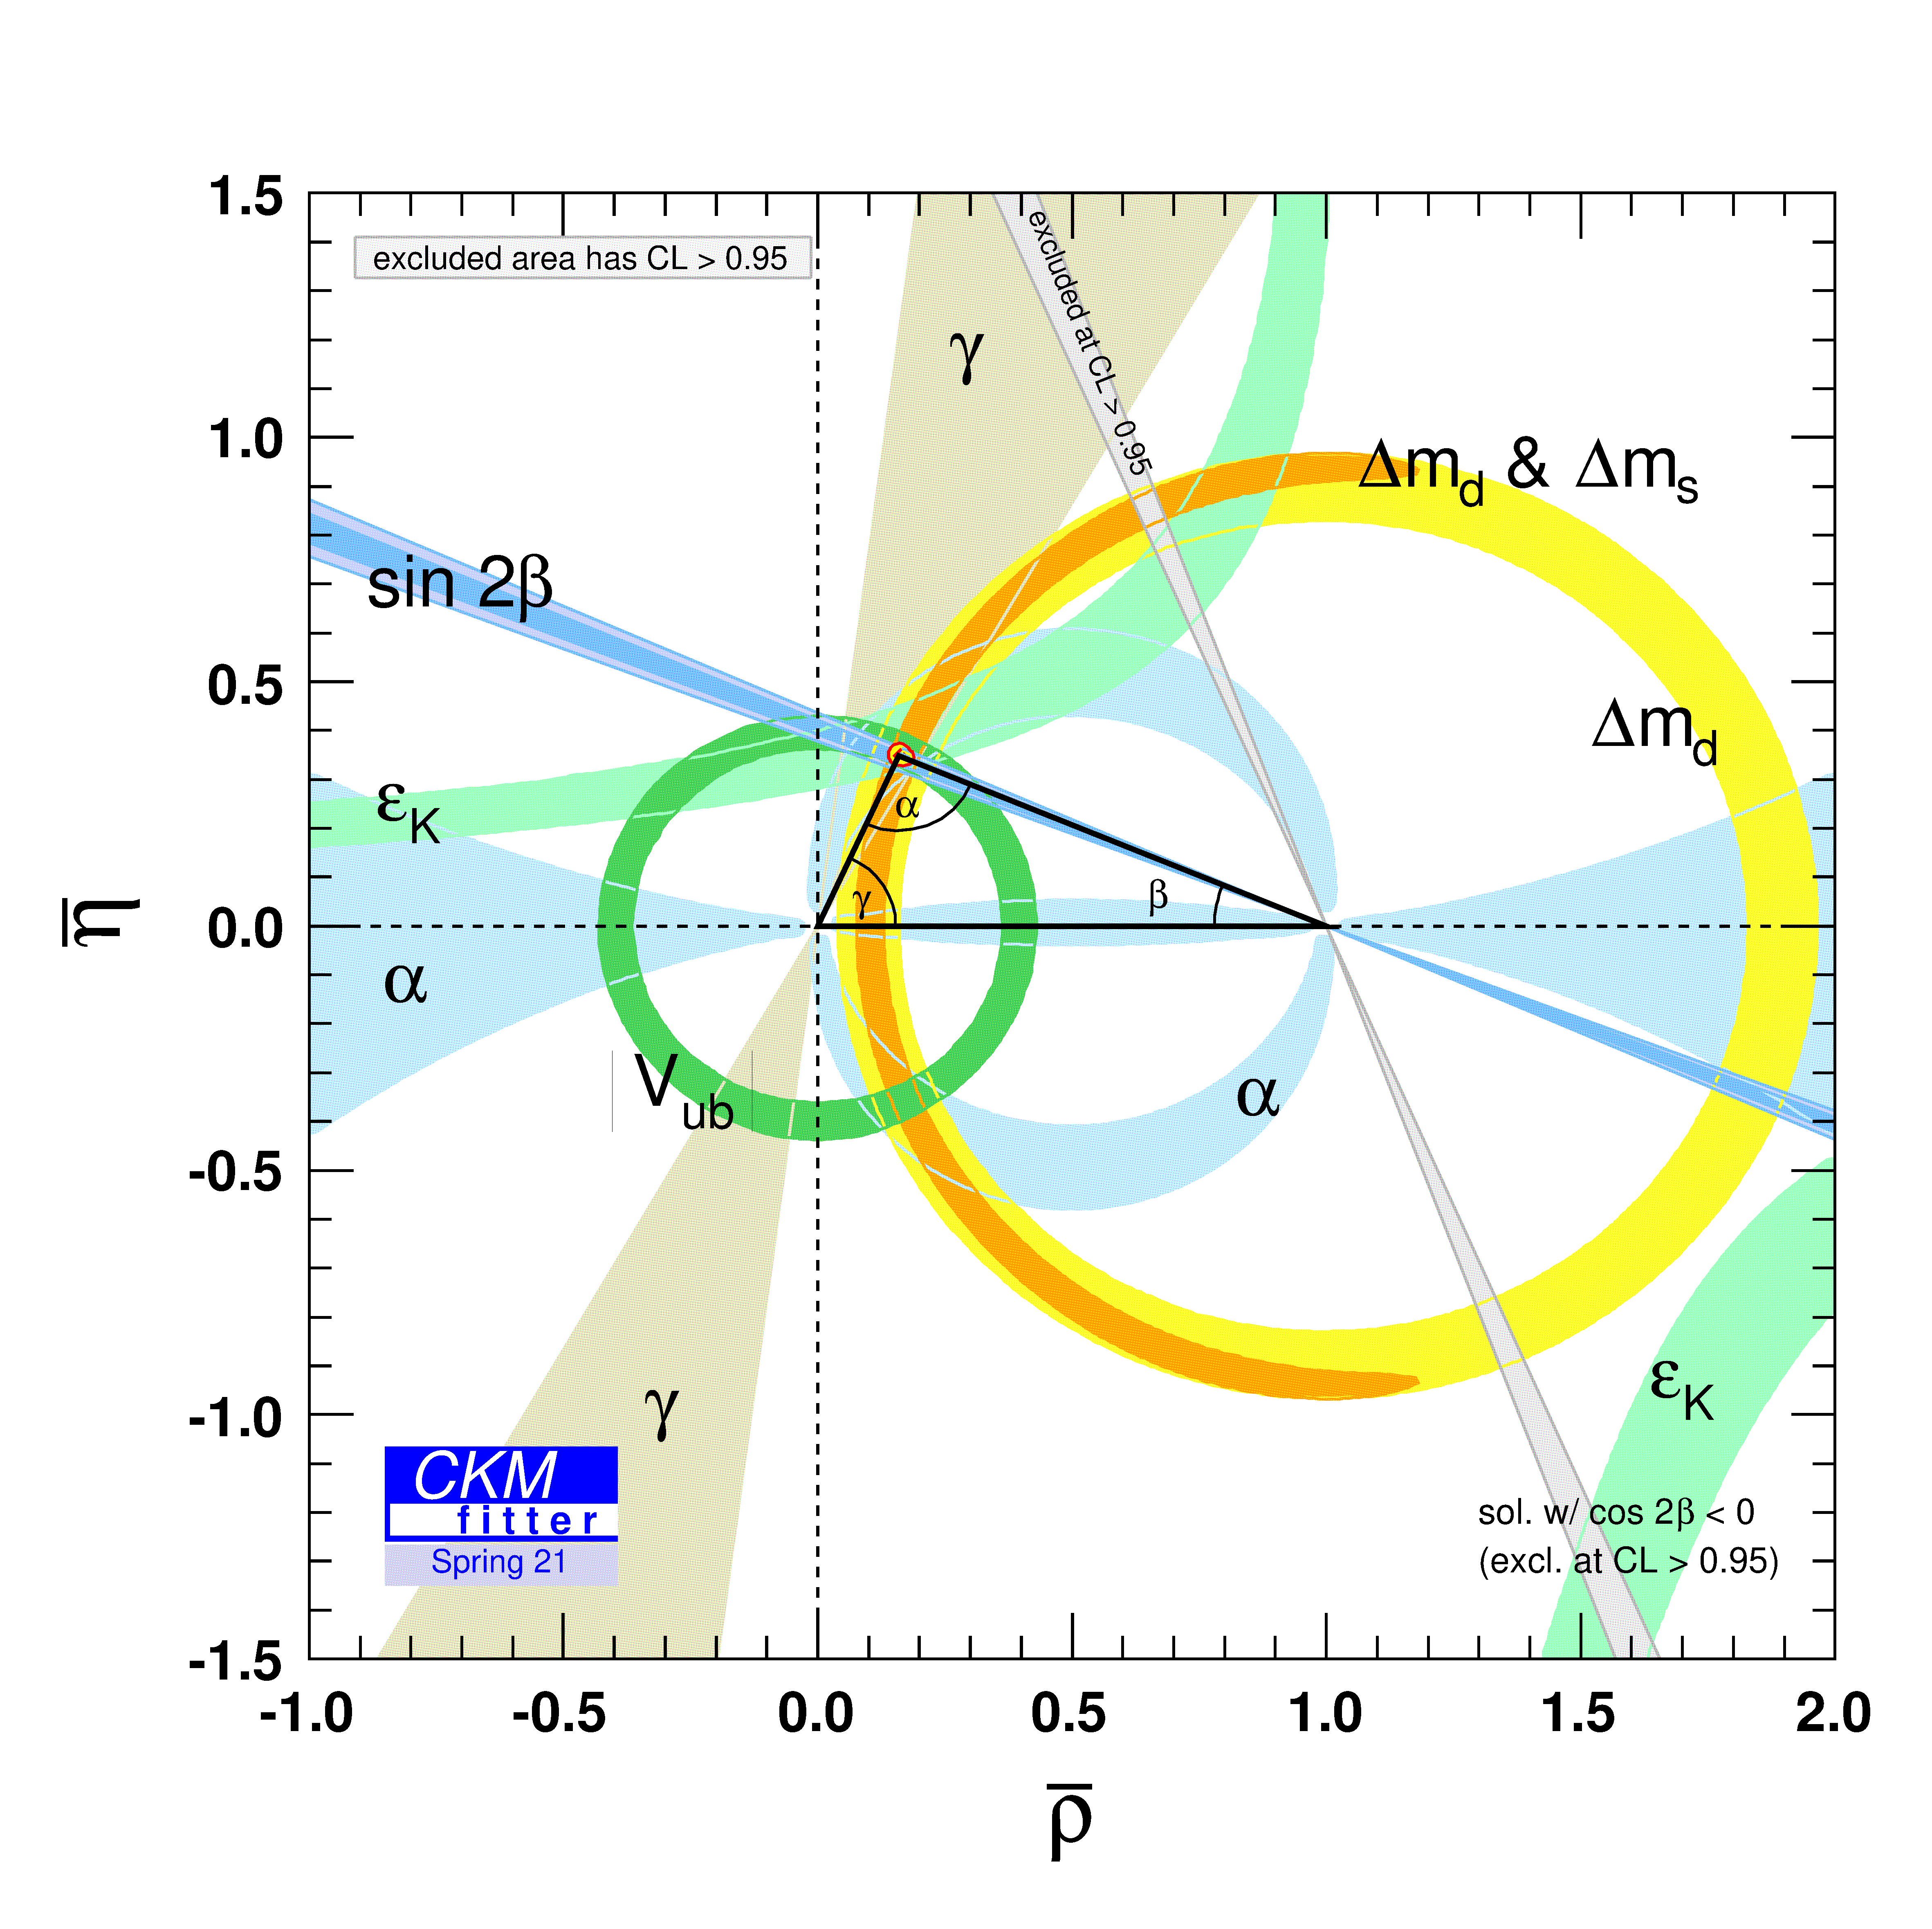
\includegraphics[width=0.85\linewidth]{fig//chap02-theory/triangle.png}
    \caption{CKMfitter global constraints on the unitarity triangle \cite{CKMfitter}. Shaded areas correspond to 95\% CL}
    \label{fig:triangle}
\end{figure}

\subsection{The $V_{cb}$ element}

\subsection{Measurement of $|V_{cb}|$ with B mesons semileptonic decays}

\paragraph*{Inclusive measurement}

\paragraph*{Exclusive measurement}


\section{The Top quark}
\subsection{Top pairs production at LHC}
\paragraph*{Extra jets}
\subsection{Top quark decay}
\subsection{Measurement of $|V_{cb}|$ with top pairs semileptonic decays}